\documentclass[letterpaper,hyper]{THG_RFC}

% Fonts
\usepackage{lmodern} % times / lmodern / mathpazo / palatino
\usepackage[scaled=.95]{helvet}
\usepackage{courier}

% Path to figures, plots
\graphicspath{{./pics/}{./plots/}}

% Code snippets
\usepackage{listings}
\def\lstsetc{\lstset{language=C,
  numbers=left,
  xleftmargin=20pt,
  numberstyle=\tiny\color{gray},
  stepnumber=1,
  showspaces=false, 
  showstringspaces=false,
  breaklines=true,
  basicstyle=\footnotesize\ttfamily,
  stringstyle=\itshape,
  commentstyle=\itshape\bfseries,
  morekeywords={main, size_t, malloc, free,
    hsize_t, hid_t, herr_t,
    H5VL_class_value_t,
    H5VL_attr_class_t,
    H5VL_dataset_class_t,
    H5VL_datatype_class_t,
    H5VL_file_class_t,
    H5VL_group_class_t,
    H5VL_link_class_t,
    H5VL_object_class_t,
    H5VL_async_class_t,
    H5VL_class_t
    }
  }
}


% Title, author, etc
\title{Virtual Object Layer}
\author{Mohamad Chaarawi}
\author{Quincey Koziol}
\date{September 16, 2014}
\rfcversion{2014-09-16.v3}
\revision{January 9, 2012}{First Draft circulated internally.}
\revision{March 9, 2012}{Update and circulate internally and externally.}
\revision{August 28, 2014}{Update with new framework changes.}
\revision{September 16, 2014}{Update with new features.}

%% Start the document
\begin{document}

%% Title
\maketitle

%% Abstract
\begin{abstract}
This RFC describes a new abstraction layer within the HDF5 library that enables different methods for accessing data and objects that conforms to the HDF5 data model. This new layer, called Virtual Object Layer (VOL), is similar to the Virtual File Layer (VFL) abstraction where different Virtual File Drivers (VFD) can be plugged in to access data in the file in different ways; however the VOL layer would be at a higher level, to allow abstract operations on objects rather than blocks of bytes. Several plugins developed already will show how the VOL abstraction would work with forms of data storage outside the typical HDF5 file paradigm.
\end{abstract}

\section{Introduction}
The HDF5 data model is composed of two basic objects, groups and datasets. The data model in itself is very powerful and widely used by many applications, including High Performance Computing (HPC) applications. The HDF5 library has an internal abstraction layer called the Virtual File Layer that the library calls after it translates the HDF5 data model and object API calls to operation on blocks of bytes. The operations on those blocks of bytes are abstracted out into drivers so that we do not limit users to one underlying implementation. Several drivers are already implemented and shipped with the HDF5 library such as the POSIX (sec2) driver, MPI-I/O driver, and a memory (core) driver.

The main challenge currently in HDF5 is not in the data model itself, but in the native HDF5 single file format that has performance issues that vary widely over different platforms and has some limitations where all objects actually have to be accessible locally. Furthermore, in parallel applications, file access by several processes has to be coordinated in order to maintain strict consistency semantics to avoid file corruption. In addition, the emergence of new tiered storage architectures and object storage file systems renders the current HDF5 library in need of major implementation changes to leverage such architectures.
To address those concerns, we have been working on a new abstraction layer inside the HDF5 library called the Virtual object layer (VOL). The VOL intercepts all HDF5 API calls that could potentially access objects in the file and forwards those calls to a plugin ``object driver''. The plugins could actually store the objects in variety of ways. A plugin could, for example, have objects be distributed remotely over different platforms, provide a raw mapping of the model to the file system, or even store the data in other file formats (like native netCDF or HDF4 format). The user still gets the same data model where access is done to a single HDF5 ``container''; however the plugin object driver translates from what the user sees to how the data is actually stored. Having this abstraction layer maintains the object model of HDF5 and would allow much better usage of new object storage file systems that are targeted for Exascale systems. 

A solid prototype for the VOL has already been implemented and used in several research projects, internally and externally. It was a key component to the FastForward~\cite{ffwd} project. However, all the work that has been done so far on the VOL was research oriented. Production is the next step to integrate this layer into the mainstream HDF5 library. The VOL implementation is in a solid prototype state that is tested daily, but a good amount of work is needed to make the VOL production ready in terms of code reviews, documentation, and support. We expect the production version of the VOL work to be a big step forward for the HDF5 library that will create new partnerships with storage vendors or users that are looking to implement new VOL plugins or users who would use existing plugins.

\section{Requirements}
The following presents a set of requirements for the VOL framework:
\begin{enumerate}
\item All HDF5 API routines that could potentially modify the HDF5 file/container should map to a VOL callback. Since the VOL plugins are implementing possible a new file format, all modifications to the container should be handed to the plugins themselves to do.
\item All HDF5 API routines that do not modify the container, but just provide memory space utilities to the application (like property lists, dataspaces, etc...) should work uniformly across all plugins. 
\item Implementing a VOL plugin should not require any change to the HDF5 library unless the plugin is an internal plugin that modifies the current native file format. 
\item Current applications, third party libraries, or tools that use the HDF5 library with the native file format should not require any change to work properly with the VOL addition.
\item Performance of applications without the VOL changes should not change. The VOL framework will introduce additional function calls to every HDF5 API call that maps to through the VOL interface, but that should be detrimental to performance.
\item Applications, third party libraries, and tools that only use the HDF5 public routines and objects should work as expected with any correct and fully implemented plugin. Performance may and probably will vary across the different plugins.
\item The VOL framework should allow plugins to be stackable on top of each other, and should allow implementation of plugins that use 2 or more different plugins. It is the plugin developer's  responsibility though to correctly implement such plugins.
\item Plugin developers should not be required to implement the full VOL functionality for a specific plugin if the intended use of that plugin is a subset of the HDF5 data model and features. For example, if a user just intends to access HDF5 datasets, it should be sufficient to develop a plugin that implement container and dataset operations in that container. Other advanced functionality of the HDF5 data model should not be required if they will not be used.
\item The HDF5 library and VOL framework should allow for new functionality or services specific to certain plugins to be added to the library and handed down to the plugin through the HDF5 library from the application.
\item Applications should be allowed to select a default plugin to use at runtime (with and environment variable possibly) or library configure time so that applications using HDF5 need not be modified to use different plugins than the native plugin.
\item VOL plugins that can be installed on a system as a shared library should be detected and loaded by the HDF5 library if the application requests their use.
\end{enumerate}

\section{Design/Architecture}
To implement a VOL interface capable of accepting any plugin a developer wishes to add, a modular design has to be put in place, similar to how the VFL interface in HDF5 is designed to accept different VFDs. The VOL is a higher level abstraction than the VFL abstraction. The following figure shows where the VOL is layered and how the data is accessed in the file:

\begin{figure}[ht!]
\centering
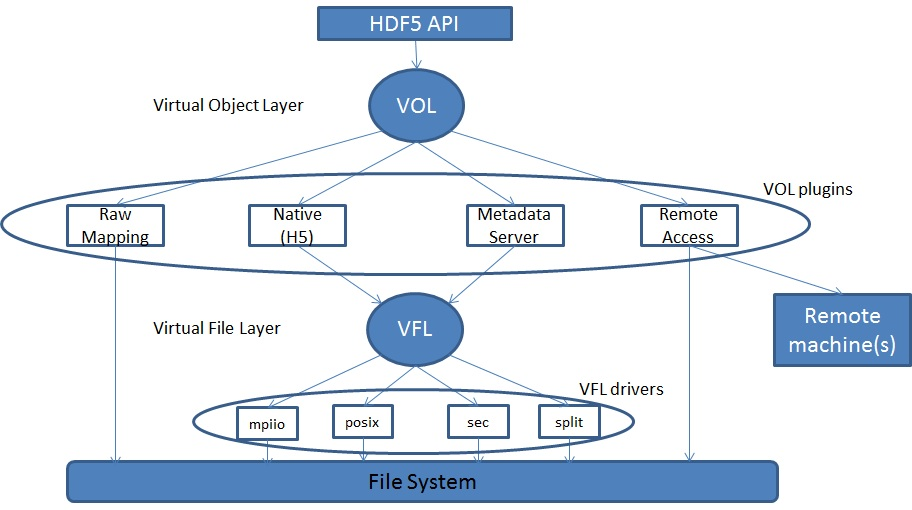
\includegraphics[width=170mm]{pics/vol-arch.jpg}
\caption{Overall VOL architecture.}
\label{fig:vol-arch}
\end{figure}

\subsection{The VOL Callback Structure}
Each VOL plugin is an instance of the following structure:

{\lstsetc
\begin{lstlisting}
/* Class information for each VOL driver */
typedef struct H5VL_class_t {
    H5VL_class_value_t value;
    const char *name;
    herr_t  (*initialize)(hid_t vipl_id);
    herr_t  (*terminate)(hid_t vtpl_id);
    size_t  fapl_size;
    void *  (*fapl_copy)(const void *info);
    herr_t  (*fapl_free)(void *info);

    /* Data Model */
    H5VL_attr_class_t          attr_cls;
    H5VL_dataset_class_t       dataset_cls;
    H5VL_datatype_class_t      datatype_cls;
    H5VL_file_class_t          file_cls;
    H5VL_group_class_t         group_cls;
    H5VL_link_class_t          link_cls;
    H5VL_object_class_t        object_cls;

    /* Services */
    H5VL_async_class_t         async_cls;
    herr_t (*optional)(void *obj, hid_t dxpl_id, void **req, va_list arguments);
} H5VL_class_t;
\end{lstlisting}
}

The VOL public structure separates Data Model operations from Service operations. Data Model operations are those that operate on files, groups, dataset, etc... Those operations are furthermore grouped in their respective ``class'' structure. For example the file class consists of function pointers for plugins to implement operations on the file itself (H5F API operations). Service operations are those that provide services for users that are not related to the data model specifically. Asynchronous operations, for example, are a service that most plugins can implement, so we add a class for it in the VOL structure. If a service becomes generic enough and common between many plugins, a class for it should be added in the VOL structure. However, many plugins can/will provide services that are not shared by other plugins. A good way to support these services is through an optional callback in the VOL structure which can be a hook from the API to the plugin that provides those services, passing any necessary arguments needed without the HDF5 library having to worry about supporting that service. A similar API operation to allow users to use that service will be added. This API call would be similar to an ``ioctl'' call where any kind of operation can be supported and passed down to the plugin that has enough knowledge from the user to interpret the type of the operation. 
The VOL User Guide will discuss the VOL structure in much more detail and provide examples on how to support/implement the classes/callbacks.

\subsection{Calling in the VOL layer}
The VOL intercepts all HDF5 API calls that potentially modify data on disk. Calls to one of these API functions only run sanity checks on the arguments passed in, and then immediately call the associated VOL callback for the API function. Operations, such as creating a group or retrieving a hyperslab from a dataset, will be captured and routed through the selected plugin that knows how the data is actually stored and capable of producing the results needed by the operations. For example, a call to H5Dcreate would be implemented within the HDF5 library as:

{\lstsetc
\begin{lstlisting}
H5Dcreate(hid_t loc_id, const char *name, hid_t type_id, hid_t space_id, hid_t lcpl_id, hid_t dcpl_id, hid_t dapl_id) {
	/* Check arguments */
	check_location (loc_id);
	check_type (type_id);
	check_dataspace (space_id);
	check_property_lists (lcpl_id, dcpl_id, dapl_id);

	/* call the corresponding callback for H5Dcreate */
	result = H5VL_dataset_create (...); /* will route the operation to the plugin at the intermediate VOL layer */
	/* return result to user (yes the dataset is created, or no here is the error */
	return result;
}
\end{lstlisting}
}

The H5Dcreate call will inform the user that a dataset with the returned ID has been created in the HDF5 container being accessed with the chosen VOL plugin. Depending on the plugin selected, the H5Dcreate function might have created a dataset object in an HDF5 file, a netCDF file, a file on a remote machine, or any way a plugin is designed to create a dataset.

\subsection{Plugin Selection}
The user should be able to select the VOL plugin and possibly provide some information to the corresponding plugin. The best way to do that is through a FAPL. For each plugin registered with the HDF5 library, a FAPL routine can be added to set the VOL plugin. If we consider the MDS plugin:
{\lstsetc
\begin{lstlisting}
hid_t fapl = H5Pcreate(H5P_FILE_ACCESS);
H5Pset_fapl_mds_vol(fapl, ...);
hid_t file = H5Fcreate("foo.h5", H5F_ACC_TRUNC, H5P_DEFAULT, fapl);
H5Pclose(fapl);
\end{lstlisting}
}

This would indicate that the MDS object layer plugin is to be used. All accesses to objects within the file opened using that FAPL would be routed through the MDS plugin.
In addition to plugins for the VOL class that will be added in the HDF5 library, any developer may write their own customizable plugin and tell the HDF5 library to use it at runtime. The plugin should be registered using:
{\lstsetc
\begin{lstlisting}
hid_t H5VLregister(H5VOL_class_t *cls)
\end{lstlisting}
}
The {\tt cls} parameter is a structure containing function pointers to the routines that implement all the callback routines the VOL class specifies. For more information on creating and using VOL plugins, please refer to the VOL user guide.

\subsection{Plugin Examples}
\subsubsection{Different File Format Plugins}
We mentioned earlier that a developer could design a plugin such that the file that stores data on disk could be of different format than the H5 format. This is very important to users that would like to use the HDF5 API and data model, but also desire the portability to use their files across different libraries or would like to access data from pre-existing files that are not in the H5 format. 

The plugin, which understands the HDF5 data model and how the data is stored, will do the necessary ``translation'' needed for this kind of model. The following figure explains more on how this is achieved:

\begin{figure}[ht!]
\centering
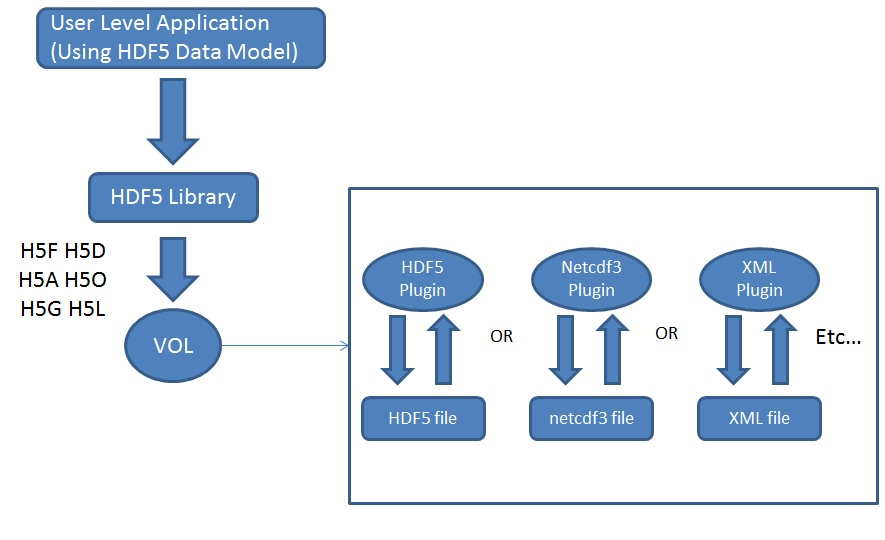
\includegraphics[width=170mm]{pics/plugin-formats.jpg}
\caption{Plugins with different underlying file formats.}
\label{fig:formats}
\end{figure}

\subsubsection{Raw Format Plugin}
The flexibility of the virtual object layer provides developers with the option to abandon the one file, binary format like the native HDF5 implementation. A ``raw'' file format could map HDF5 objects (groups, datasets, etc ...) to file system objects (directories, files, etc ...). The entire set of raw file system objects created would represent one HDF5 container as opposed to one HDF5 file with the native plugin. The actual mapping between all HDF5 objects to file system objects is subject to further research.

This plugin would allow the PLFS package~\cite{plfs} to be applied to applications that use the HDF5 API, where access seems to be done to a single file from the high level, but is mapped by the raw plugin to multiple files/directories for performance benefits that were demonstrated by PLFS.

\subsubsection{Remote Access Plugin}
The current HDF5 implementation requires applications to access a single HDF5 file that is also local on the file system where the application resides. A remote VOL plugin would allow access to files located remotely. The plugin could have an HDF5 server module located where the HDF5 file resides and listens to incoming requests (HDF5 operations that are routed through the VOL) from a remote process. 

Remote visualization is an important use case for this plugin. Large, remote datasets are very expensive to migrate to the local virtualization system. It would be faster to just enable in situ virtualization to remotely access the virtualization data using the HDF5 API. This is however not possible at the moment with the native implementation for HDF5 as the file is required to be present locally.

\subsubsection{MDS Plugin}
The MDS plugin uses the proposed strategy in the Independent Metadata RFC~\cite{mds}, which allows processes in HPC applications to call HDF5 operations that modify metadata independently (the current HDF5 semantics require those calls to be collective). The MDS is a set-aside process that manages access to the file's metadata to avoid corruption from simultaneous access by several processes. The design strategy is explained in details in the Independent Metadata RFC.

The MDS strategy puts all HDF5 metadata in a separate file, different than the raw data file. Only the designated MDS process will read/write data to that file. All HDF5 calls made by other processes that potentially need to access the metadata or raw data file must go through the MDS process to serialize access to the metadata and acquire the necessary locks for proper synchronization. Figure~\ref{fig:mds} shows the flow of the operation from the VOL layer to the MDS plugin:

\begin{figure}[ht!]
\centering
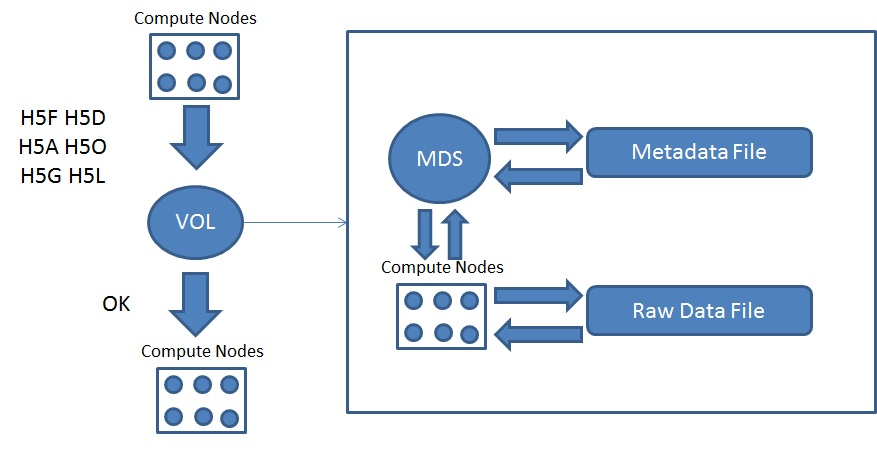
\includegraphics[width=170mm]{pics/plugin-mds.jpg}
\caption{Metadata server plugin.}
\label{fig:mds}
\end{figure}

All H5F, H5D, H5A, H5O, H5G, and H5L API calls are mapped to MDS specific implementations. An H5Dopen call, for example, would forward the parameters of the routine to the MDS that actually opens the dataset and returns the ID to the calling process along with some metadata for that dataset. The user gets back the ID of the opened dataset. An H5Dwrite call would ask the MDS process for a shared lock on the dataset being written to, to avoid having another process modify the metadata of the dataset, and then would actually write the data from the API call.
\clearpage
\subsection{Interchanging and Stacking VOL plugins}
Accessing a file created with a different VOL plugin than the one it was created with would be a valid operation as long as the underlying file format is the same. This would be the user’s responsibility to ensure that the different plugins are interchangeable. 

It would be also possible to stack VOL plugins on top of each other. This notion is similar to the idea of the split VFD, where underneath the split VFD itself, two file drivers would be used, one for the file storing the metadata and another for raw data. Some stackings make sense and others would be erroneous. For example, stacking the native HDF5 plugin on top of a non-HDF5 backend plugin does not make sense and is erroneous. Figure~\ref{fig:stack} showes a stacking of the remote plugin, where data is distributed remotely, on top of the native h5 plugin, where servers that store the data at remote locations use the h5 file format.

\begin{figure}[h!]
\centering
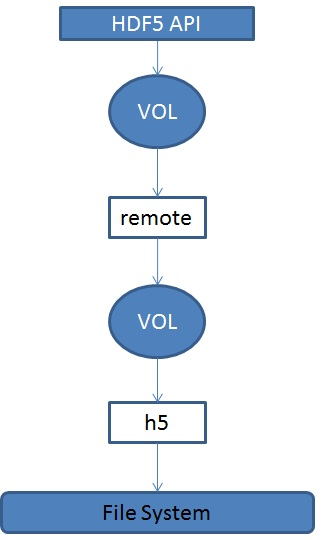
\includegraphics[width=90mm]{stacked.jpg}
\caption{Stacked VOL plugins.}
\label{fig:stack}
\end{figure}

Another useful design option is to allow a mirroring plugin, where the HDF5 API calls are forwarded through a mirror plugin to two or more VOL plugins. This is an extention to the stacking feature. Figure~\ref{fig:mirror} shows an example of a VOL mirror that maps HDF5 API calls to an h5 backend plugin and an XML backend plugin:

\begin{figure}[h!]
\centering
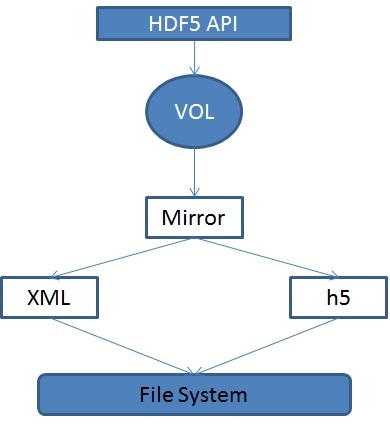
\includegraphics[width=90mm]{mirrored.jpg}
\caption{Mirrored VOL plugins.}
\label{fig:mirror}
\end{figure}

Another possible VOL plugin could be a statistics plugin that just gathers information on HDF5 API calls and records statistics associated with the number of calls to a specific API functions and corresponding parameters. This plugin would be very useful for profiling purposes. The statistics plugin would be stacked on top of another VOL plugin that actually performs the required access to the file.
\clearpage
\section{Implementation}
The VOL class structure consists of data structure(s) that contain configuration variables that are set by each plugin and a collection of function pointers that maps all HDF5 API operations that access data on disk to the plugin's corresponding implementations. Internally, each plugin is free to implement the underlying storage of objects in any way desired. The main goal is that the user still gets the same HDF5 API and data access model no matter which plugin is used. This section highlights some implementation and feature details.  

\subsection{VOL Callbacks}
A VOL plugin is initialized based on the user selection with a file access property list API call or the default that the library chooses. The plugin is an instance of the VOL class and contains an implementation for the function callbacks specified by the VOL class. 

The VOL class includes all the higher level logical callbacks that potentially touch data (metadata or raw data) on disk. All the API routines should map to one of those callbacks. The HDF5 API is too large however to have a 1 to 1 mapping from API routines to VOL callbacks, so we introduce the notion of a generic function call that developers could use to implement certain API routines that do not map to one of the VOL callbacks. This is similar to the UNIX {\tt ioctl()} routine.

The HDF5 library currently does not support nonblocking I/O operations. However, since it is a very desirable feature, future versions of the library most probably will add nonblocking routines. In order to be able to support those API routines and not to double the number of VOL callback routines, we made all VOL callbacks nonblocking compatible, by adding an HDF5 request parameter to all VOL callbacks. If the high level operation issued by the user is nonblocking, then the request would just be forwarded to the VOL plugin and the plugin itself would be responsible to support the nonblocking behavior. If the high level operation is a blocking operation, then a non-active request is forwarded to the plugin which detects that the request is inactive and implements the operation in a blocking behavior. 

One could argue that the interface can be simplified by having, for example, a common open routine for all objects (like the {\tt H5Oopen}) routine. We found however that having  a common interface would be detrimental to performance in certain plugin implementations, since it would require querying the VOL plugin twice, once for looking up the object location and once for opening the object. Having an optional callback for every object and a generic one would solve this issue. The VOL layer would check if the specific object callback is implemented in the VOL plugin, and if it is not, it would fall back to the generic object callback routine. This way we do not sacrifice performance for generality.

Another design issue comes to mind when looking at the large set of functions, and that is whether to lump all the functions together into one data structure as the VOL class, or to have a more object oriented approach, where we can either have a general class that contains all common functions, and then children of that class that contain functions specific to certain HDF5 objects, or for each object have a set of callbacks that are specific to that object. The current design chosen seems to be a good middle ground between generality and readability/maintainability.

\subsection{Internal vs. External Plugins}
Developers can implement their VOL plugin as a plugin internal to the HDF5 library or an external plugin. Internal plugins are ones that rely heavily on internal and private HDF5 functionality like the native and metadata server plugins. They are required to ship with the HDF5 library to be used by applications. External plugins on the other hand are ones that are implemented outside of the HDF5 library and applications link with to use. Those plugins do not require using private HDF5 functionality. They can however use public HDF5 features.

External plugins can be provided by the applications themselves or as a third party library, i.e. not provided by the HDF5 library nor the application. Third party plugins should be installed on the system to be used as a shared library or a DLL. HDF5 will attempt to load the plugin if the application requests its use. This is similar to Filter plugins~\cite{filters}. Refer to the VOL user guide for more detailed information on how to develop and use VOL plugins.

\subsection{{\tt H5Ocopy and H5Ocompare}}
The HDF5 API has two routines that will require extra attention to be compatible with the VOL layer, and those are the object copy and compare routines:
{\lstsetc
\begin{lstlisting}
herr_t H5Ocopy( hid_t src_loc_id, const char *src_name, hid_t dst_loc_id, const char *dst_name, hid_t ocpypl_id, hid_t lcpl_id );
htri_t H5Ocompare(hid_t loc1_id, const char *name1, hid_t lapl1,  hid_t loc2_id, const char *name2, hid_t lapl2, hid_t cmppl_id, H5O_cmp_cb_t *cb_info);
\end{lstlisting}
}

If the two objects are in containers of the same type, i.e. created using the same VOL plugin, then the VOL layer would be able to detect that and forward those calls to the corresponding implementation using a designated VOL callback. This would allow different sorts of optimizations that a VOL plugin could choose to implement in order to copy or compare two objects. On the other hand, if the objects belong to two different containers, the VOL plugin would not be able to interpret an object created by a different plugin, and so a different approach needs to be considered.

Comparing two objects that belong to different types of HDF5 containers require processing independent of the VOL plugins. One way to accomplish this is to add utility routines to the VOL class to retrieve certain characteristics about an object for comparison. For example, datasets would need utility routines to retrieve the dataset name, dimensions, type, space, and elements. Once those values are retrieved for each object from each VOL plugin, the comparison operation could return the required result. The copy operation would require the same level of processing on the source object. Then using the fetched attributes, the same object is created using a create callback of the destination object's VOL plugin.

\section{Recommendation}

\section*{Revision History}
\makerevisions

%% References
\bibliographystyle{ieeetr}
\bibliography{RFC_VOL}

\end{document}
